%%%%%%%%%%%%%%%%%%%%%%%%%%%%%%%%%%%%%%%%%%%%%%%%%%%%%%%%%%%%%%%%%%%%%%
% Overview
\section{Overview}
Dialog systems, also referred to as chatbots or virtual agents are systems that can converse with a human to help with their informational needs. Dialog systems are used in a wide range of applications such as personal assistants in mobile phones, technical support services, chit chat, product enquiries, IVR systems and entertainment. Some of the popular dialog systems include Apple's Siri, Google Now, Microsoft's Cortana, Amazon's Alexa and Google's Smart Reply. Most of the dialog systems that are being used for real word applications are hand crafted by a dialog designers and also very specific to a domain. Even though using such hand crafted rules provides the flexibility to build a interpretable dialog system, it requires a great amount of effort for the dialog designer to create one from scratch for a new domain. This extra effort also transcends to scenarios where the existing chatbot's capability has to be extended or improved.

% Recent advancements in the field of neural networks has shown us that data-driven approaches outperform systems with custom hand crafted features. This has been proven for a number of NLP tasks such as part of speech tagging, named entity recognition, speech recognition, etc. This trend is now being observed in the area of building dialog systems. Research on data driven approaches for modeling dialogs have started to shadow the research around improving the traditional hand crafted dialog systems. The data driven approaches have the ability to learn to mimic a human with just access to a large corpus of conversation logs. The system learnt using data driven approaches can at best be used to provide suggestions to possible next responses or provide context based auto complete features in social media, email client or chat applications. For example, the \textit{smart reply} option in GMail. This option scans the email conversation so far and suggests three possible responses to reply with. These systems are far from performing a full fledged conversation and help accomplish user's goal.

% \begin{figure}
% \centering
%  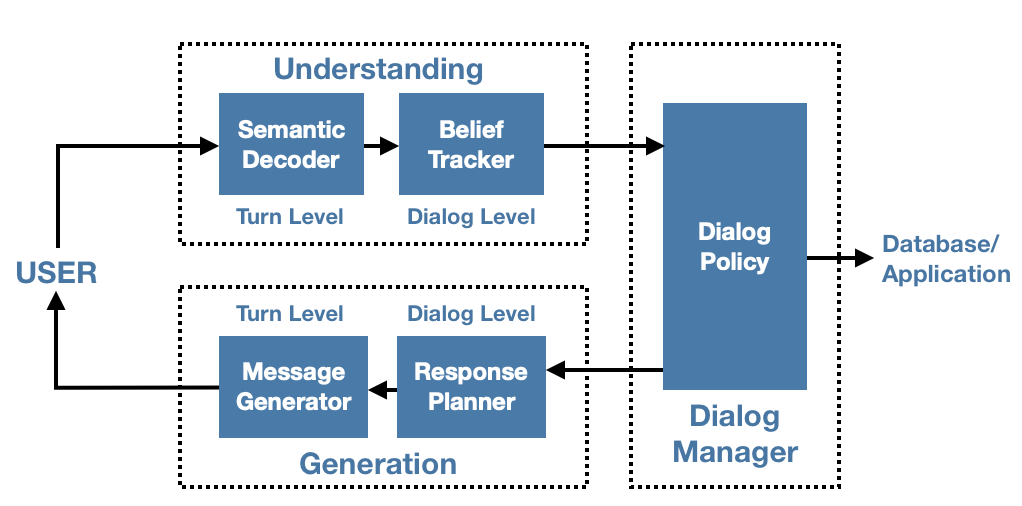
\includegraphics[width=0.9\textwidth]{assets/figures/dialog_system.png}
% \label{fig:arch}
% \caption{Architecture of Dialog System}
% \end{figure}

\begin{figure}
\centering
\begin{subfigure}{\textwidth}
 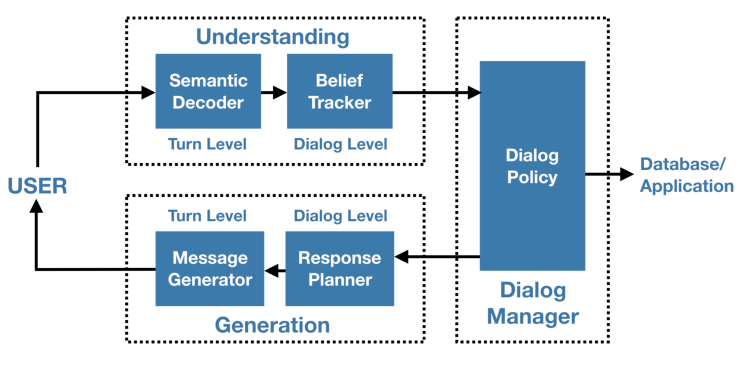
\includegraphics[width=\linewidth]{assets/figures/components.pdf}
 \caption{Multi-Component Dialog System}\label{fig:systemfull}
\end{subfigure}

\vspace*{0.5in}

\begin{subfigure}{\textwidth}
 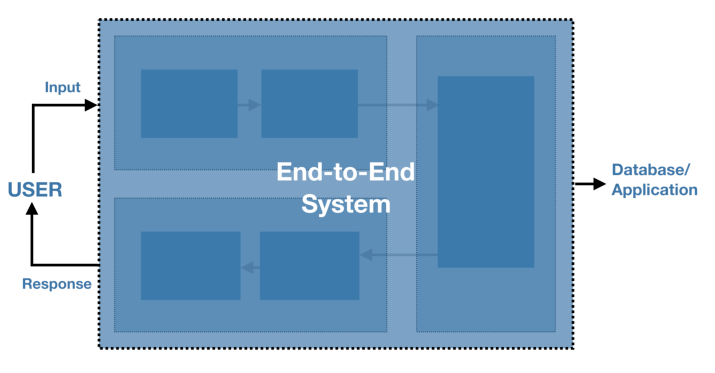
\includegraphics[width=\linewidth]{assets/figures/end2end.pdf}
 \caption{End-to-end Dialog System}\label{fig:end2end}
\end{subfigure}
\caption{Types of Dialog System Architecture}
\end{figure}

\noindent\textbf{End-to-End Learning}: A complete dialog system is comprised of several sub-modules with different functionalities. Broadly we can classify these into three primary components: 1) natural language understanding (NLU) unit, 2) dialog manager and 3) natural language generator (NLG). The architecture is shown in Figure \ref{fig:systemfull}. Each component can be either built using hand-crafted rules or can be a statistical machine learning model that learns from a provided set of examples. A complete dialog-system, which is a combination of these components, can then be partly hand-designed and partly data-driven. In some cases, the designer will choose to combine two or more components together because of the type of data that is avaliable. This bypasses the need for explicitly annotating the data to serve each component separately, but in exchange, the complexity of the module increases thereby demanding a lot more data to train. The approach where all the three components are combined together and examples of (user input in natural language, expected response in natural language) pairs are used to learn a dialog model, is referred to as \textit{end-to-end} dialog models. Note that in end-to-end learning, the intermediate output space may be defined, but examples are not annotated with expected intermediate outputs. This architecture is depicted in Figure \ref{fig:end2end}.
% While building a dialog system, the components could either be built using hand crafted rules or can also be a statistical machine learning model that learns from a provided set of examples (data-driven). A complete dialog system can thus have some components that are built using rules and some that are learnt using data driven approaches. 
% As mentioned previously, not all dialog system built needs to have all three components, in some cases, the designer can decide to combine both dialog manager and the NLG into a single modules. This way the component can be learnt by using a set of (NLU output, expected natural language response) pairs. Even though this bypasses the need for explicitly annotating the dialog manager output for each dialog exchange, the complexity of the module increases thereby demanding a lot more data to train. The approach where all the three components are combined together and examples of (user input in natural language, expected response in natural language) pairs are used to learn a dialog model, is referred to as \textit{end-to-end} dialog models. Note that in end-to-end learning, the intermediate output space may be defined, but examples are not annotated with expected intermediate outputs.

\noindent\textbf{Task-Oriented}: Application of dialog systems can be broadly categorized into two types: open domain (non-task-oriented) dialog systems and task-oriented dialog systems. The main difference between the two approaches is that, the objective of the former is usually broad and not well defined (abstract), where as the objective of the latter is narrow and well-defined. For example, the restaurant reservation domain dialogs falls under task-oriented systems. The goal could be, given a set of options (cuisine: {\em Chinese}, location: {\em East Delhi}), the system should be able to suggest the right restaurant that is acceptable by the user. A large portion of the research in data driven approaches for dialog modeling has been around open domain systems. Some examples include chit-chat and language learning. Applications such as restaurant reservation, flight booking, travel enquiry and bus enquiry belong to the task-oriented setting. One advantage of working with task-oriented dialogs is the ease of defining evaluation techniques to measure the performance of the system. The performance of the system can be measured by the percentage of conversations where the dialog system was able to help the user achieve their goal. 

Question answering systems and task-oriented dialog systems are very similar to each other. The major difference between the two is that, in question answering all details necessary to achieve the task are provided in a single shot, where as in task-oriented dialog, the user conveys information spaced throughout the converstation. In the latter it is the job of the dialog system to collect the necessary information to complete the task. These architectures also provide the ability to carry over context when switching between tasks.

\noindent\textbf{Knowledge Base in the Loop}: These are the subset of dialog systems that require access to a knowledge base to respond to user input. Some examples of knowledge bases systems are: a bus inquiry system using a KB with bus running status, a restaurant reservation system using a KB filled with restaurant information, etc. There has been a large amount of work on using databases in systems that use hand-crafted features for modeling dialog. The community has recently (in 2017) started to explore the area of learning data-driven dialog models grounded by a knowledge base.

We interact with the Knowledge Base using specially designed APIs that are task specific. These APIs will have the ability to either retrieve information or update information in the KB. Traditionally, API calls have been simple template based responses that employ slot-filling techniques for each template entry. However, the retrieval power could be increased if the APIs would become more flexible and dynamic. This would enable the selection of more precisise results and even allow simple data manipulations, such as sorting, which could aid in training the system.

Typically, to train dialog systems associated with a knowledge base, we need to annotate the knowledge base incorporation in the dialog data itself. For example, if the system is to query the KB, then the corresponding API call must be included in the dialog explicitly. This makes it difficult to create a large training corpus as general ASR systems won't be able to recognise the API call being performed and the data curator must add it manually.

% Dialog systems can be largely differentiated into two categories, namely, open domain and task-oriented.

% \noindent {\bf Open Domain}: Dialog that doesn't involve any underlying task. As a result it is not domain specific and is often broad and unstructured. For example, normal chit-chat and language learning.

% \noindent {\bf Task-Oriented}: Dialog where an agent converses with a user with the goal of accomplishing a specific task and often interact with a knowledge-base (KB). For example, a restaurant reservation agent \cite{hen2014word} will be grounded to a KB that contains the names of restaurants, and their details. 

% For instance, Mem2Seq \cite{mem2seq} exhibits satisfactory performance when tested on the training KB. It represents the dialog history and the KB knowledge as a \emph{bag of words} in a flat memory arrangement. This enables Mem2Seq to revisit each word several times, as needed, obtaining good performance. But at the same time, flat memory prevents it from capturing any surrounding context -- this deteriorates its performance rapidly when the amount of new unseen information in the KB increases, as shown in Figure \ref{fig:camrest}. On the other hand, the performance of copy augmented sequence-to-sequence network (Seq2Seq+Copy) \cite{eric2017copy}, is robust to changes in the KB, but fails to achieve acceptable task-oriented performance. It captures context by representing the entire dialog history as one continuous \emph{sequence}. However, it can be difficult for a sequence encoder to reason over long dialogs found in real-world datasets and its ability to learn the task gets hampered. 

%%%%%%%%%%%%%%%%%%%%%%%%%%%%%%%%%%%%%%%%%%%%%%%%%%%%%%%%%%%%%%%%%%%%%%
% Problem Definition
\section{Problem Definition}
The focus of this thesis will be to improve the ability of task-oriented dialog systems to generalise over its KB.
In real-world applications, the KB information could change over time. For example, (1) a KB associated with a movie ticket booking system gets updated every week based on new film releases, and (2) a restaurant reservation agent, trained with the knowledge of eateries in one city, may be deployed in other cities with an entirely different range of establishments. In such situations, the system should have the ability to conform to new-found knowledge unseen during its training. Ideally, the training algorithm must learn to disentangle the language model from the knowledge interface model. This separation will enable the system to generalize to KB modifications, without a loss in performance. 

Moreover, for achieving good progress towards the user's task, the agent must also retain the ability to draw inferences based on past utterances and the KB. Notably, we find that existing approaches either achieve this disentanglement or effective progress towards the task, but not both. 

We will also focus on enabling the system to predict the correct API call without explicit annotations. This will help us twofold: (1) we will be able to leverage larger databanks for training end-to-end dialog systems which don't have this additional KB annotation, and (2) we will be able to predict more efficient APIs to solve the task than those originally used.

To summarize, the goal of our research is to build a dialog system that takes as input (1) a large set of task-oriented conversation logs between a user and an agent/domain expert, (2) a knowledge base used to generate agent response and learn a dialog system that can mimic the agent to accomplish a user's task. 
With this goal in mind we can broadly formulate two distinct problems as follows:

\noindent{\bf Problem 1} {\em Create an end-to-end dialog system that effectively disentangles the language and knowledge models.}

The system must be capable to handle changes in the database which we will simulate using systematic adversarial attacks which mutates KB information. We will test the effectiveness of the system on three standard datasets used for task-oriented dialog -- bAbI \cite{BordesW16}, CamRest \cite{wenEMNLP2016}, and Stanford Multi-Domain Dataset \cite{Ericsigdial}. Of these, the last two are real-world datasets. We show a sample dialog and its components in Figure \ref{sampledialog}.
% We will evaluate the responses using standard metrics in the task-oriented setting.

\noindent{\bf Problem 2} {\em Enable the end-to-end system to achieve comparable performance on datasets without explicit Knowledge Base API annotations.}

The mentions datasets will have to be augmented to remove the extra annotation depicting the API information and a {\em"predict API"} signal should be inserted in its exact place. The system will be evaluated using the same metrics as before and the objective will be to acheive the same performance as the model trained in the first problem definition.

\begin{figure}
\centering

 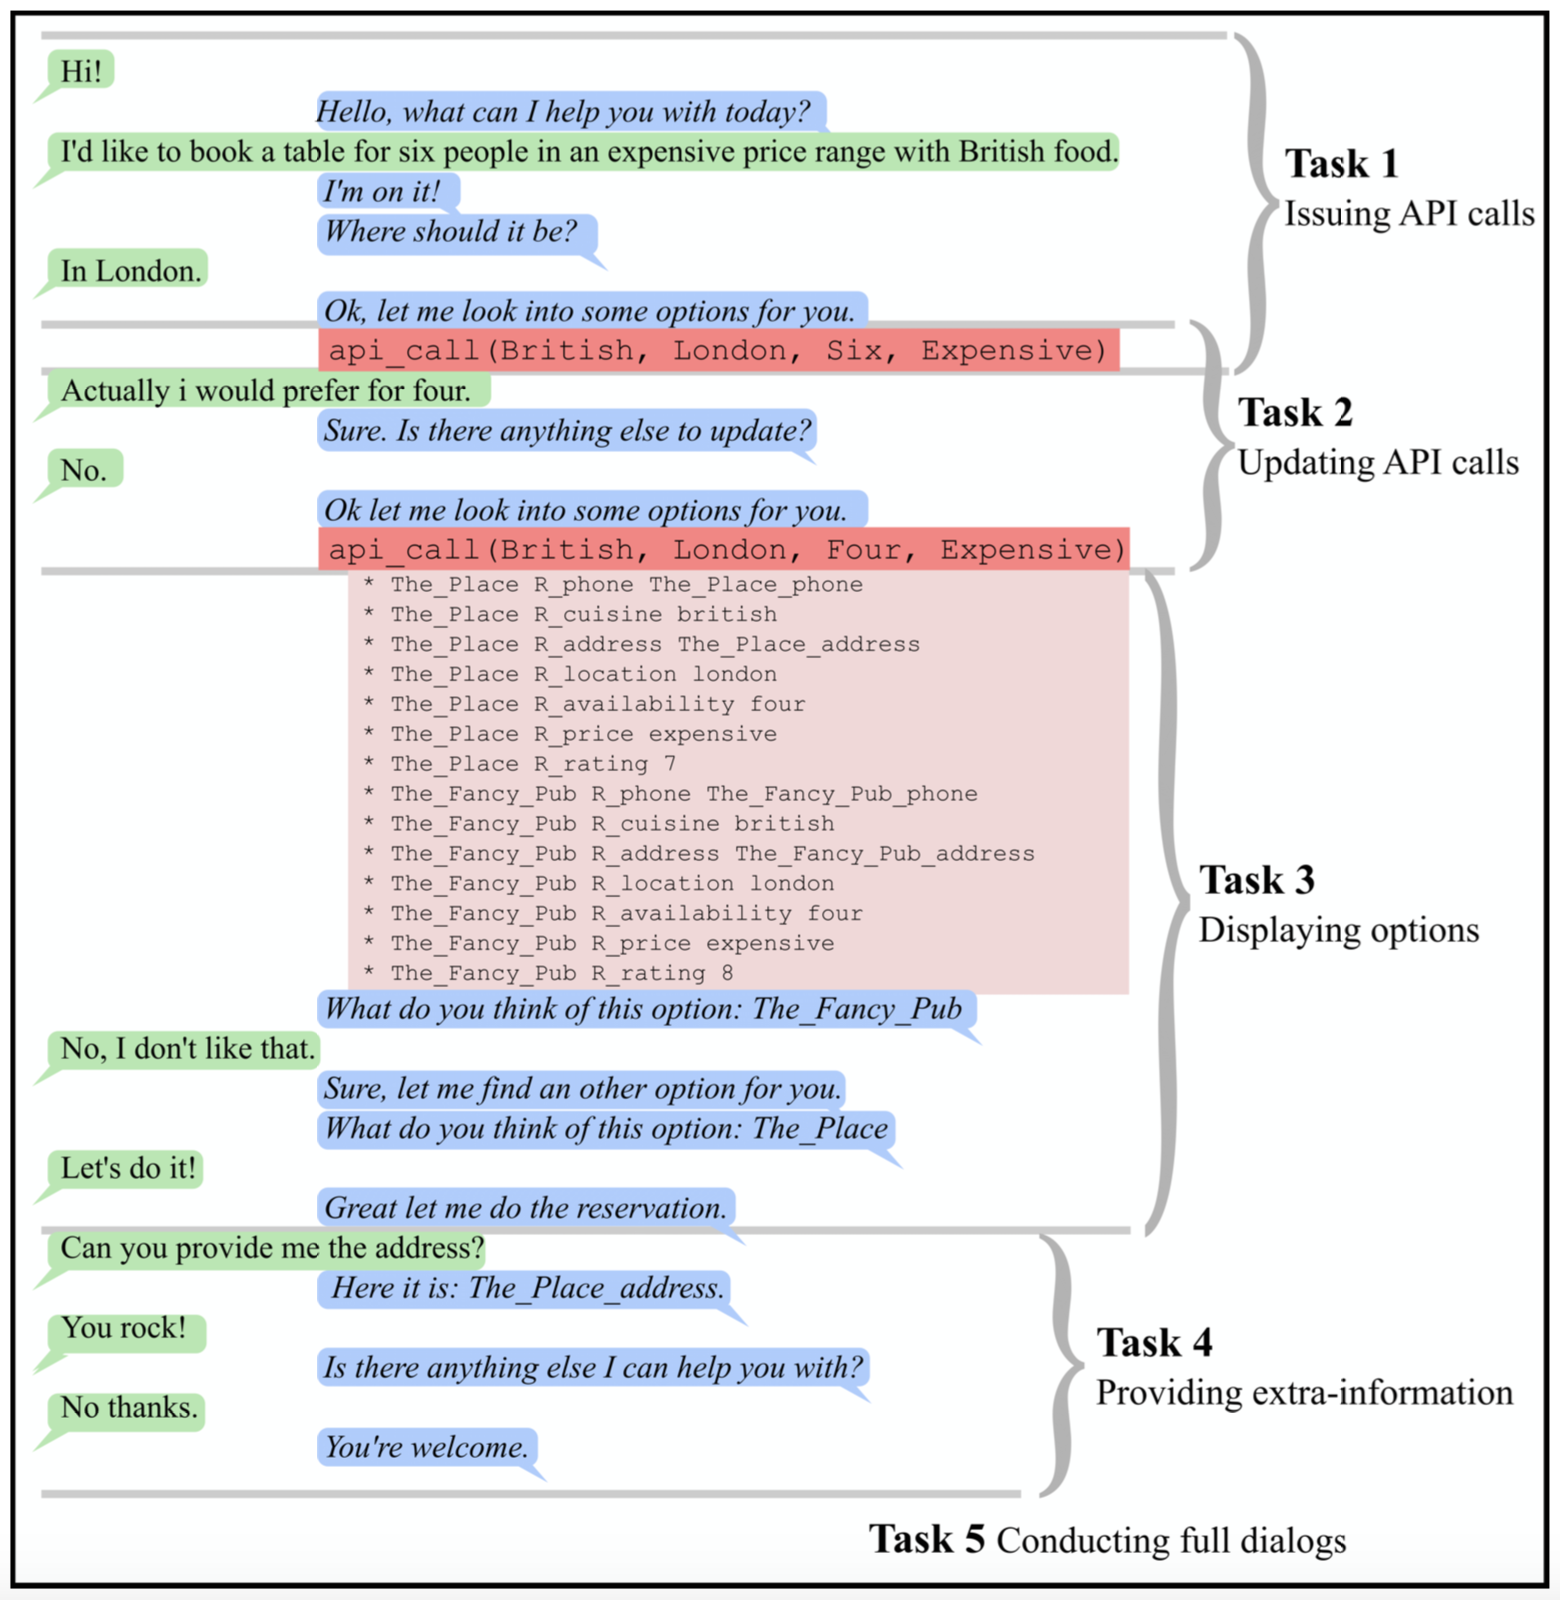
\includegraphics[width=\linewidth]{assets/figures/dialog_sample.png}

\caption{A breakdown of tasks in bAbI dialog. User queries are in green, system responses in blue, APIs in red along with their fetched KB results. Figure credits \cite{bordes2016learning}}
\label{fig:sampledialog}
\end{figure}

%%%%%%%%%%%%%%%%%%%%%%%%%%%%%%%%%%%%%%%%%%%%%%%%%%%%%%%%%%%%%%%%%%%%%%
% Motivation
\section{Motivation}
In this section, we motivate our problem by clearly defining the gap between what the state-of-the-art, data-driven approaches for dialog learning are capable of and what it takes to build a usable end-to-end task-oriented dialog system that requires a knowledge base.

\noindent \textbf{Why cant already proven non-task-oriented models be used?}

While end-to-end non-task-oriented (open domain) dialog systems are being used in real world applications \cite{smartreply}, designers still prefer using hand crafted rules for modeling task-oriented dialogs. The main reason for success in non-task-oriented setting is that, models have largely been evaluated (and applied) in scenarios where, given the conversation so far the system is expected to predict just the immediate next response. Such modeling requires the system to learn a language model and a mapping from the context to the response. But in case of task-oriented settings, the requirements/expectations are much more. It is not just required to generate the next utterance based on the context, but understand the global picture of what the task is, what all details are necessary to finish the task, what is the optimal way or strategy to request for missing details, and then decide what the next utterance should be. Also, in chit chat bot (non-task-oriented) making a mistake in a single turn is not very costly, where as in flight booking system (task-oriented) making a single mistake (mis-interpreting a source city) could turn out to be very costly. Even though a large section of real world applications such flight booking, technical service support, basic medical consultations fall under this category, there has been very little focus so far.

In addition to task-oriented setting, when a knowledge base is added into the loop, the system should now also be able to learn when to query a knowledge base, how to incorporate the results from the knowledge base into the conversation. Also, such KB-centric task-oriented dialogs generally need specially annotated data which is not easily available as compared to unannotated dialogs which used to train open domain systems. This makes the problem much harder and harder to generalise. Hence models that have been proven to work on non-task-oriented systems cannot be used for task-oriented applications.\\

\noindent \textbf{How is dialog data collected for data-driven modelling?}

Most datasets used in open domain dialog systems are obtained using Automatic Speech Recognistion (ASR) techniques. Here a recording of a conversation between two individuals can easily be transcribed and added to the large data corpora. This ease of data collection and large datasets has invited a lot of research interest in open domain dialog. Task-oriented dialog requires specific annotation for it to be usable, such as interaction with the Knowledge Base via an API and the results themselves. Difficultly to annotate such instances automatically has led to scarce data reserves and has forced researchers to fabricate data of their own.

\noindent \textbf{Limitations of state-of-the-art task-oriented approaches}

There has been very little progress made end-to-end task-oriented dialogs, as most of the proposed approaches has been around using hand crafted rules to either build the entire system, or to define the structured space of each sub-components output. The only work published so far on end-to-end task-oriented conversation has the following limitations:
\begin{enumerate}
\item Both the human and the agent utterances in the dataset are fabricated using rules. This simulated dataset is very simple compared to human to human conversation logs.
\item The learned model is unable to generalise over a Knowledge Base and performance suffers greatly whenever KB modifications are made. It has no support for field values that have never been encountered so far (OOVs).
\item The system performance is has acceptable accuracy on non-task-oriented evaluation metrics, but the performance is very poor on task-oriented evaluation metrics
\item The system is unable to learn simple patterns (that are exhibited in the train corpora) required to perform a task-oriented dialog, such as not repeating already suggested options and sorting based on a particular field.
\item The system proposed has a very limited view of the knowledge base. It assumes that it can only perform simple {\em SELECT} operation with {\em WHERE} clauses over the knowledge base
\end{enumerate} 

%%%%%%%%%%%%%%%%%%%%%%%%%%%%%%%%%%%%%%%%%%%%%%%%%%%%%%%%%%%%%%%%%%%%%%
% Contributions
\section{Contributions}

To address our first problem statement, we propose \sys, a novel network that effectively disentangles the language and knowledge models, and also achieves state-of-the-art performance on three existing datasets. 

To achieve this, \sys\ makes three design choices. 
First, \sys\ uses an encoder-decoder architecture so that it can stitch the next utterance one word at a time as compared to a typical retrieval based model which selects a certain response from a fixed set of responses. 
Second, it encodes the conversational input as a {\em bag of sequences} (\textsc{BoSs}) memory, in which the input representation is built at two levels of abstraction. The \emph{higher level} flat memory encodes the KB tuples and utterances to facilitate effective inferencing over them. The \emph{lower level} encoding of each individual utterance and tuple is constructed via a sequence encoder (Bi-GRU). This enables the model to maintain the sequential context surrounding each token, aiding in better interpretation of unseen tokens at test time. 
Third, we augment the standard cross-entropy loss used in dialog systems with an additional loss term to encourage the model to only copy KB tokens in a response, instead of generating them via the language model. This combination of sequence encoding and additional loss (along with dropout) helps in effective disentangling between language and knowledge. 

We find that \sys\ is competitive or significantly better on standard metrics in all datasets as compared to state-of-the-art baselines. We also introduce {\em adversarial attacks} in which we systematically increase the percentage of previously unseen entities in the KB. We summarise these attacks as our {\em knowledge adaptability} (KA) evaluation. We find that \sys\ is highly robust across all percentage levels in all the standard metrics. We also report a human-based evaluation and find that \sys\ responses are frequently rated higher than other baselines.

To address the second problem statement, we extend \sys\ and add a novel RL-decoder which generates the required API call at a fixed turn of the dialog. We train the system using a buffer containing valid API calls and do a mix of off-policy and on-policy sampling. We use a pseudo-reward for learning which is computed using a combination of precision and recall on the retrieved results and the gold system response KB entities. We were successfully able to achieve similar accuracies to the original \sys\ model trained on the fully annotated dataset.

Overall, our contributions are:

\begin{enumerate}
 \item We propose \sys, a novel architecture to disentangle the language model from knowledge incorporation in task-oriented dialogs.
 \item We introduce a {\em knowledge adaptability} evaluation to measure the ability of dialog systems to scale performance to unseen KB entities.
 \item Our experiments show that \sys\ is competitive or significantly better, measured via standard metrics, than the existing baselines on three datasets.
 \item We extend the \sys\ architecture and add a novel RL-based API generator which matches state-of-the-art performance on modified datasets which lack explicit API annotation.
\end{enumerate}

Our work addressing the first problem statement was published as a full paper in the Proceedings of the 2019 Conference of the North American Chapter of the Association for Computational Linguistics: Human Language Technologies (NAACL-HLT 2019). \url{https://www.aclweb.org/anthology/papers/N/N19/N19-1126/}.

We release our code and {\em knowledge adaptability} (KA) test sets for further use by the research community. \url{ https://github.com/dair-iitd/BossNet}. We also release our extended code base along with the modified test sets. \url{ https://github.com/NikhilGupta1997/BossNet-RL}.

